\documentclass[14pt]{article}
\usepackage{listings}
\usepackage{color}
\usepackage{graphicx}
\usepackage{setspace}
\usepackage{mathtools}
\usepackage{amsmath}

\definecolor{dkgreen}{rgb}{0,0.6,0}
\definecolor{gray}{rgb}{0.5,0.5,0.5}
\definecolor{mauve}{rgb}{0.58,0,0.82}

\lstset{frame=tb,
  language=Java,
  aboveskip=3mm,
  belowskip=3mm,
  showstringspaces=false,
  columns=flexible,
  basicstyle={\small\ttfamily},
  numbers=none,
  numberstyle=\tiny\color{gray},
  keywordstyle=\color{blue},
  commentstyle=\color{dkgreen},
  stringstyle=\color{mauve},
  breaklines=true,
  breakatwhitespace=true
  tabsize=3
}

\begin{document}
\title{\huge \textbf{Synchronization Mechanisms Lab Assignment} }
\date{\today}
\maketitle
\begin{center}
\vspace{30 mm}

\title{\huge \textbf{Student: Brinzan Florinel-Razvan}}
\\\vspace{10 mm}
\title{\huge Calculatoare si tehnologia informatiei (limba romana)}
\\\vspace{10 mm}
\title{\huge \textbf{C.R 3.1 A}}
\\\vspace{10 mm}
\title{\huge \textbf{Anul 3}}
\date{}
\maketitle

\newpage
\end{center}

\section{Problema 1 -- Producator-Consumator}

\vspace{4 mm}

\subsection{Enuntul problemei}

\vspace{2 mm}


\textbf{--- Implementați problema Producator-Consumator folosind:}

\begin{enumerate}
\item \textbf{semafoare}
\item \textbf{monitoare }
\item \textbf{lacate}
\end{enumerate}

\textbf{Pe scurt}, exista mai multi\textbf{ producatori si consumatori}. \textbf{Fiecare producator va produce elemente (numere) distincte intr-un interval de numere dat si le va plasa intr-un buffer de marime fixa. Rolul consumatorilor este acela de a consuma elemente din buffer. }

---\textbf{Probleme ce pot aparea:}

\begin{itemize}
\item Producatorul vrea sa adauge un element in buffer in momentul in care acesta este full.
\item Consumatorul vrea sa consume un element din buffer in momentul in care acesta este gol.
\end{itemize}

\textbf{Pentru a evita aceste 2 probleme trebuie sa blocam producatorul sa mai produca elemente cat timp buffer-ul este plin si sa blocam consumatorul sa mai consume elemente din buffer cat timp acesta este gol.}

\subsection{Implementarea problemei in Java}

\subsubsection{\textbf{Utilizarea semafoarelor}}

\vspace{2 mm}

--- In implementarea acestei probleme am creat 4 clase: clasa PCSemafor, clasa Producator, clasa Consumator si clasa Main.


\begin{enumerate}
\item \textbf{Clasa PCSemafor} detine cele \textbf{doua semafoare} prin intermediul carora \textbf{producatorii pot adauga elemente in buffer} (in limita spatiului disponibil - nu se poate suprascrie un element din buffer daca acesta nu a fost inca consumat) iar \textbf{consumtorii pot extrage elemente }( in limita stocului din buffer - nu se poate consuma un element ce a fost consumat anterior). \textbf{Un consumator nu poate extrage elemente din buffer daca acesta e "gol"} (are doar elemente ce au fost consumate de firul curent sau alte fire de executie) \textbf{deoarece este blocat de "semafor-consumator",iar producatorul nu poate adauga elemente in buffer daca acesta este "plin"} ( are doar elemente ce nu au fost consumate inca) \textbf{fiindca este blocat de "semafor-producator".}



---\textbf{In clasa PCSemafor sunt implementate metodele de producere si consumare a elementelor buffer-ului. }



\begin{itemize}
\item \textbf{Metoda\textit{ void append(int)}} -- \textbf{prin aceasta metoda Producatorul adauga elemente in buffer. }\textbf{Cat timp counter-ul (numarul de elemente neconsumate) este mai mic decat capacitatea buffer-ului se vor produce noi elemete} (acestea vor suprascrie elemente deja consumate din buffer si counter-ul ce numara elementele neconsumate va creste).\textbf{ Daca counter-ul va avea valoarea capacitatii buffer-ului  atunci firul de executie  va fi blocat pana se va apela metoda \textit{release()}. }\textbf{In momentul in care se adauga un nou element in buffer semaforul consumatorului primeste \textit{release()}.}
\end{itemize}

 \textbf{PSEUDOCOD}
 \begin{lstlisting}
		cat timp counter == CAPACITATE executa
			blocheaza semafor_producator				

		buffer[newest] <- element primit ca parametru
		newest <- ((newest + 1) % CAPACITATE)
		counter <- (counter + 1)
		elibereaza semafor_consumator
\end{lstlisting}


\begin{itemize}
\item \textbf{Metoda\textit{ int take()}} --\textbf{ prin aceasta metoda Consumatorul extrage elemente din buffer.}\textbf{ Cat timp counter-ul este mai mare decat 0 insemana ca exista elemente neconsumate in buffer, deci consumatorul le poate extrage} ( incepand cu  cel mai vechi element introdus)\textbf{.Daca counter-ul va avea valoarea 0 atunci firul de executie va fi blocat pana se va apela metoda \textit{release()} pentru semafor-consumator. In momentul in care se extrage un element din buffer semaforul producatorului primeste \textit{release()} - elibereaza permis-ul, returnandu-l semaforului.}
\end{itemize}


 \textbf{PSEUDOCOD}
 \begin{lstlisting}
	    element <- 0
		cat timp counter == 0 executa
			blocheaza semafor_consumator	

		element <- buffer[oldest];
		oldest <- (oldest + 1) % CAPACITATE;
		counter <- (counter - 1)
		elibereaza semafor_producator
		returneaza element
\end{lstlisting}

\newpage

\item \textbf{Clasa Producator} extinde clasa \textbf{Thread} si \textbf{suprascrie metoda \textit{"run()"}}.Aceasta clasa are ca membrii de tip data elementele ce vor fi  initializate cu valorile date ca parametri in constructor. \textbf{Clasa contine un constructor cu parametri, o metoda prin care se returneaza numarul de elemente produse si metoda\textit{ run() }ce apeleaza metoda \textit{append(int)} din clasa PCSemafor pentru a adauga elemente in buffer.}



\begin{itemize}
\item \textbf{Metoda\textit{ int getCounter()} returneaza numarul de elemente produse de firul curent.}
\end{itemize}


\begin{itemize}
\item \textbf{Metoda \textit{void run()} suprascrie metoda "run()" din clasa Thread. Metoda "\textit{run()}" din clasa Producator are rolul de a genera elementul (un nr intreg din intervalul [min, max) ) si a-l introduce in buffer prin intermediul metodei\textit{ append(int)} din clasa PCSemafor. La final se incrementeaza numarul de elemente produse de firul curent, se afiseaza numarul producatorului si numarul elementului adaugat in buffer.}
\end{itemize}


 \textbf{PSEUDOCOD}
 \begin{lstlisting}
	    element <- min
		cat timp (element % nr_fireP) != nr_fir executa
			element <- element +1
		
		cat timp (element < max) executa
			adauga element in buffer
			nr_elemente_produse <- nr_elemente_produse +1
			afiseaza ce producator a produs elementul
			element <- element + nr_fireP
\end{lstlisting}

\item \textbf{Clasa Consumator} extinde clasa \textbf{Thread} si \textbf{suprascrie metoda "\textit{run()}"}. Aceasta clasa are ca membrii de tip data elementele ce vor fi  initializate cu valorile date ca parametri in constructor. \textbf{Clasa contine un constructor cu parametri, o metoda prin care se returneaza numarul de elemente consumate si metoda\textit{ run()} ce apeleaza metoda\textit{ take()} din clasa PCSemafor pentru a extrage elemente din buffer.}


\begin{itemize}
\item \textbf{Metoda int getCounter() returneaza numarul de elemente consumate de firul curent.}
\end{itemize}


\begin{itemize}
\item \textbf{Metoda void\textit{ run()} suprascrie metoda "\textit{run()}" din clasa Thread. Metoda "\textit{run()}" din clasa Consumator are rolul de a extrage elemente din buffer prin intermediul metodei \textit{take(}) din clasa PCSemafor. La final se incrementeaza numarul de elemente consumate de firul curent, se afiseaza  numarul consumatorului si numarul elementului consumat din buffer.}
\end{itemize}


 \textbf{PSEUDOCOD}
 \begin{lstlisting}
		iterator <- min
		element <- 0
		
		cat timp(iterator % nr_fireC) != nr_fir executa
			iterator <- iterator + 1

		cat timp (iterator < max) executa
		
			element <- cel mai vechi element din buffer
			nr_elemente_consumate <- nr_elemente_consumate + 1
			afiseaza ce consumator a consumat elementul
			iterator <- iterator + nr_fireC
		}
\end{lstlisting}

\item \textbf{Clasa Main }contine metoda "\textbf{\textit{main()}}" in care \textbf{sunt instantiati producatorii si consumatorii.} Aceasta clasa contine 4 variabile statice - finale ce reprezinta\textbf{ numarul de producatori (\textit{NR-PRODUCATORI})},\textbf{ numarul de consumatori (\textit{NR-CONSUMATORI}),} \textbf{limita inferioara si superioara a intervalului de numere/produse (\textit{MINN} respectiv \textit{MAXN})} . \textbf{Clasa Main} contine un obiect de tip \textbf{PCSemafor} ce reprezinta buffer-ul de elemente care va fi dat ca parametru \textbf{tuturor firelor de executie (producatori si consumatori)}.

\begin{itemize}
\item In \textbf{metoda \textit{main()}} sunt create thread-urile (producatorii si consumatorii) si este apelata metoda "\textbf{\textit{start()}}" ce pune in executie thread-urile. \textbf{Fiecare producator / consumator primeste ca parametrii numarul de producatori/consumatori, numarul sau de identificare, limita inferioara si superioara a intervalului de numere(produse) si buffer-ul de numere(produse).} La final se afiseaza numarul de elemente produse de fiecare producator si numarul de elemente consumate de fiecare consumator.
\end{itemize}
\end{enumerate}

 \textbf{PSEUDOCOD metoda main()}
 \begin{lstlisting}
 
        NR_PRODUCATORI <- 10
        NR_CONSUMATORI <- 5
        MINN <- 0
        MAXN <- 50
        iterator <- 0
        Producator producatori[]
        Consumator consumatori[]
        PCSemafor buffer

        
		pentru iterator de la 0 la NR_PRODUCATORI - 1 executa
			producatori[iterator] <- new Producator(NR_PRODUCATORI, iterator, MINN, MAXN, buffer)
			start producatori[iterator]

		pentru iterator de la 0 la NR_CONSUMATORI - 1 executa
			consumatori[iterator] <- new Consumator(NR_CONSUMATORI, iterator, MINN, MAXN, buffer)
			start consumatori[iterator]
		
		pentru iterator de la 0 la NR_PRODUCATORI - 1 executa
				join producatori[iterator]

		pentru iterator de la 0 la NR_CONSUMATORI - 1 executa
				join consumatori[iterator]

		pentru iterator de la 0 la NR_PRODUCATORI - 1 executa
			afiseaza Producatorul X a produs Y elemente
		
		pentru iterator de la 0 la NR_CONSUMATORI - 1 executa 
			afiseaza Consumatorul X a consumat Y elemente

\end{lstlisting}


\subsubsection{\textbf{Utilizarea lacatelor}}

\vspace{2 mm}

---In implementarea acestei probleme am creat \textbf{4 clase}:  clasa \textbf{PCLock}, clasa \textbf{Producator}, clasa  \textbf{Consumator} si clasa \textbf{Main}.

\vspace{4 mm}

---Clasele \textbf{Producator}, \textbf{Consumator} si \textbf{Main} au ramas neschimbate (cu precizarea ca in locul obiectului \textbf{PCSemafor} se va folosi un obiect de tip \textbf{PCLock}. \textbf{Descrierea acestor clase este prezentata mai sus.}

\vspace{4 mm}

---Clasa \textbf{PCLock} detine lacatul, conditiile si cele doua metode (\textbf{\textit{append}} si \textbf{\textit{take}}) prin intermediul carora producatorii pot adauga elemente in \textbf{buffer} (in limita spatiului disponibil - nu se poate suprascrie  un element din buffer daca acesta nu a fost inca consumat) iar consumtorii pot extrage elemente ( in limita stocului din \textbf{buffer} - nu se poate consuma un element ce a fost consumat anterior). Un consumator nu poate extrage elemente din \textbf{buffer} daca acesta e "\textbf{gol}" (are doar elemente ce au fost consumate de firul curent sau alte fire de executie) deoarece va intra in bucla "\textbf{while}" si va trebui sa astepte pana va primi semnalul dat de metoda \textbf{\textit{signalAll().}} Un producator nu poate adauga elemente in buffer daca acesta este "\textbf{plin}" ( are doar elemente ce nu au fost consumate inca) fiindca va intra in bucla "\textbf{while}" si va trebui sa astepte pana va primi semnalul dat de metoda\textbf{\textit{ signalAll()}}. La intrarea in cele 2 metode lacatul se va inchide si va fi deblocat doar la iesirea din metoda.


\begin{itemize}
\item \textbf{Metoda \textit{void append(int)}} -- \textbf{Prin aceasta metoda Producatorul adauga elemente in buffer}. \textbf{Cat timp counter-ul este mai mic decat capacitatea buffer-ului se vor produce noi elemete (acestea vor suprascrie elemente deja consumate din buffer si counter-ul ce numara elementele neconsumate va creste). Daca counter-ul va avea valoarea capacitatii buffer-ului atunci firul de executie va intra in bucla while si va astepta sa fie notificat. In momentul in care se adauga un element in buffer se apeleaza metoda \textit{signalAll()} ce trezeste toate firele de executie. La apelarea acestei metode lacatul se va bloca si va fi deblocat doar la iesirea din metoda.}
\end{itemize}

 \textbf{PSEUDOCOD}
 \begin{lstlisting}
		blocheaza lacatul
		cat timp (counter == CAPACITATE) executa
			asteapta
		buffer[newest] <- element
		newest <- (newest + 1) % CAPACITATE
		counter <- counter + 1
		trezeste firele
		deblocheaza lacatul
\end{lstlisting}

\begin{itemize}
\item \textbf{Metoda\textit{ int take()} -- Prin aceasta metoda Consumatorul extrage elemente din buffer. Cat timp counter-ul este mai mare decat 0 insemana ca exista elemente neconsumate in buffer, deci consumatorul le poate extrage ( incepand cu cel mai vechi element introdus).Daca counter-ul va avea valoarea 0 atunci firul de executie va astepta sa fie notificat. In momentul in care se extrage un element din buffer se apeleaza metoda \textit{signalAll()} ce trezeste toate firele de executie. La apelarea acestei metode lacatul se va bloca si va fi deblocat doar la iesirea din metoda.}
\end{itemize}


 \textbf{PSEUDOCOD}
 \begin{lstlisting}
	    element <- 0
		blocheaza lacatul
		cat timp (counter == 0) executa
			asteapta

		element <- buffer[oldest]
		oldest <- (oldest + 1) % CAPACITATE
		counter <- counter - 1
			
		trezeste firele
		deblocheaza lacatul
		returneaza element
\end{lstlisting}

\newpage

\subsubsection{\textbf{Utilizarea monitoarelor}}

\vspace{2 mm}

---In implementarea acestei probleme am creat \textbf{4 clase}:  clasa \textbf{PCMonitor}, clasa \textbf{Producator}, clasa  \textbf{Consumator} si clasa \textbf{Main}.

\vspace{4 mm}

---Clasele \textbf{Producator}, \textbf{Consumator} si \textbf{Main} au ramas neschimbate (cu precizarea ca in locul obiectului \textbf{PCSemafor} se va folosi un obiect de tip \textbf{PCMonitor}. \textbf{Descrierea acestor clase este prezentata mai sus.}

\vspace{4 mm}

---Clasa \textbf{PCMonitor} detine cele \textbf{doua metode sincronizate (\textit{append} si \textit{take})} \textbf{prin intermediul carora producatorii pot adauga elemente in buffer} (in limita spatiului disponibil - nu se poate suprascrie un element din buffer daca acesta nu a fost inca consumat) \textbf{iar consumtorii pot extrage elemente} ( in limita stocului din buffer - nu se poate consuma un element ce a fost consumat anterior). Un consumator nu poate extrage elemente din buffer daca acesta e "\textbf{gol}" (are doar elemente ce au fost consumate de firul curent sau alte fire de executie) deoarece va intra in bucla "\textbf{while}" si va fi adormit, iar producatorul nu poate adauga elemente in buffer daca acesta este "\textbf{plin}" ( are doar elemente ce nu au fost consumate inca) fiindca va intra in bucla "\textbf{while}" si va fi adormit. Asteptarea firelor se va incheia in momentul in care va fi apelata metoda \textbf{\textit{notifyAll()}} ce \textbf{va trezi toate firele care asteapta pe monitorul obiectului}.

\begin{itemize}
\item \textbf{Metoda\textit{ synchronized void append(int)} }--\textbf{ Prin aceasta metoda Producatorul adauga elemente in buffer. Cat timp counter-ul este mai mic decat capacitatea buffer-ului se vor produce noi elemete (acestea vor suprascrie elemente deja consumate din buffer si counter-ul ce numara elementele neconsumate va creste). Daca counter-ul va avea valoarea capacitatii buffer-ului atunci firul de executie va intra in bucla while si va astepta sa fie notificat. In momentul in care se adauga un element in buffer se apeleaza metoda\textit{ notifyAll()} ce trezeste toate firele care asteapta pe monitorul obiectului}.
\end{itemize}


 \textbf{PSEUDOCOD}
 \begin{lstlisting}
		cat timp (counter == CAPACITATE) executa
			asteapta
		buffer[newest] <- element
		newest <- (newest + 1) % CAPACITATE
		counter <- counter + 1
		trezeste firele
\end{lstlisting}

\begin{itemize}
\item \textbf{Metoda \textit{synchronized int take()} -- Prin aceasta metoda Consumatorul extrage elemente din buffer. Cat timp counter-ul este mai mare decat 0 insemana ca exista elemente neconsumate in buffer, deci consumatorul le poate extrage ( incepand cu  cel mai vechi element introdus).Daca counter-ul va avea valoarea 0 atunci firul de executie va astepta sa fie notificat. In momentul in care se extrage un element din buffer se apeleaza metoda \textit{notifyAll()} ce trezeste toate firele care asteapta pe monitorul obiectului.}
\end{itemize}


 \textbf{PSEUDOCOD}
 \begin{lstlisting}
	    element <- 0
		cat timp (counter == 0) executa
			asteapta

		element <- buffer[oldest]
		oldest <- (oldest + 1) % CAPACITATE
		counter <- counter - 1
			
		trezeste firele
		returneaza element
\end{lstlisting}

\subsection{Rezultate, Scenarii posibile si descrierea output-ului}

---\textbf{Sunt 3 scenarii posibile: }

\begin{enumerate}
\item \textbf{Producatorii} si \textbf{Consumatorii} produc si consuma elemente simultan si nu se va ajunge niciodata la limitele buffer-ului ( 0 elemente respectiv 5 elemente ) - \textbf{scenariu mai deloc intalnit.}
\item \textbf{Producatorii} \textbf{vor aveam momente cand vor vrea sa produca elemente si nu va mai fi spatiu disponibil in buffer} ( vor fi doar elemente neconsumate si nu le vor putea suprascrie). In acest caz  producatorii trebuie opriti din a mai produce elemente ( folosirea metodelor \textbf{\textit{acquire(), await(), wait(), lock()}} ). \textbf{Producatorii vor incepe sa produca elemente numai atunci cand bufer-ul are cel putin un element deja consumat ce va putea fi suprascris).}



\begin{itemize}
\item Implementarea solutiilor pentru acest scenariu:
\end{itemize}


\begin{center}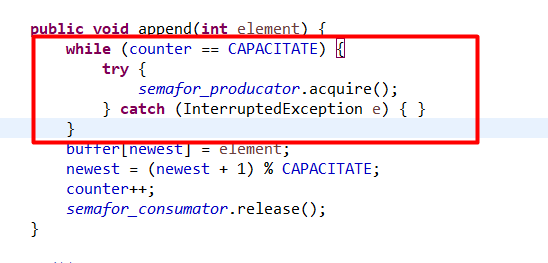
\includegraphics[height=1.70 in, width = 3.4 in]{prodStop3.png}
\end{center}

===========================================

\begin{center}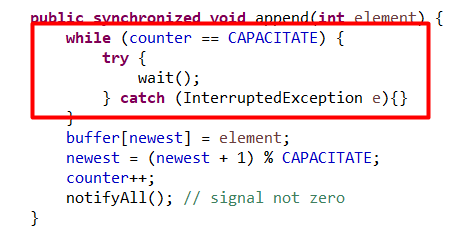
\includegraphics[height=1.7 in, width = 3.5 in]{prodStop2.png}
\end{center}

===========================================

\begin{center}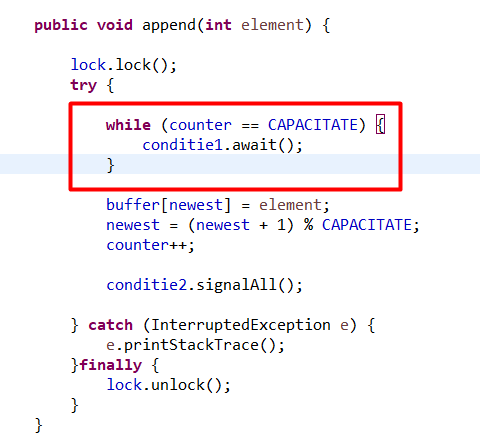
\includegraphics[height=3 in, width = 3.5 in]{prodStop.png}
\end{center}

\item \textbf{Consumatorii vor avea momente cand vor dori sa consume elemente din buffer dar buffer-ul s-ar putea sa fie gol} (are doar elemente deja consumate). In acest caz consumatorii trebuie opriti din a mai consuma elemente, iar acest lucru este posibil prin apelarea metodelor  \textbf{\textit{acquire(), await(), wait(), lock()}}. \textbf{Consumatorii vor incepe sa consume din nou elemente cand cel putin un producator va pune in buffer un elemnt nou ( atunci vor fi "treziti/deblocati" consumatorii ce asteapta).}
\end{enumerate}

\begin{itemize}
\item Implementarea solutiilor pentru acest scenariu:
\end{itemize}

\begin{center}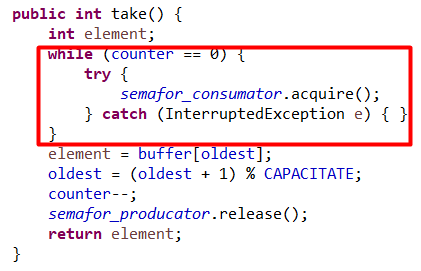
\includegraphics[height=2.3 in, width = 3.5 in]{consStop.png}
\end{center}

===========================================

\begin{center}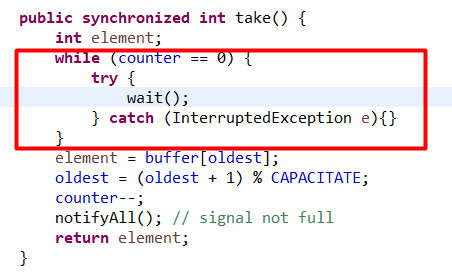
\includegraphics[height=2.3 in, width = 3.5 in]{consStop2.png}
\end{center}

===========================================

\begin{center}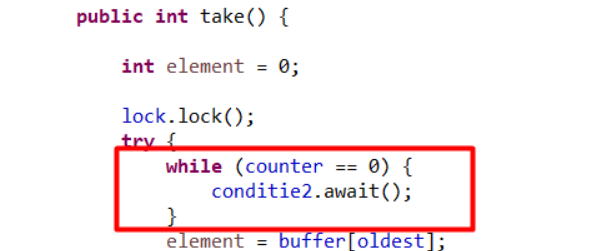
\includegraphics[height=1.5 in, width = 3.5 in]{consStop3.png}
\end{center}

\newpage

\begin{itemize}
\item \textbf{In consola se afiseaza numarul producatorului si ce element a produs precum si numarul consumatorului si ce element a consumat.}
\end{itemize}


\begin{itemize}
\item \textbf{La final se calculeaza totalul de elemente produse de fiecare producator si totalul de elemente consumate de fiecare consumator.}
\end{itemize}
.

\begin{center}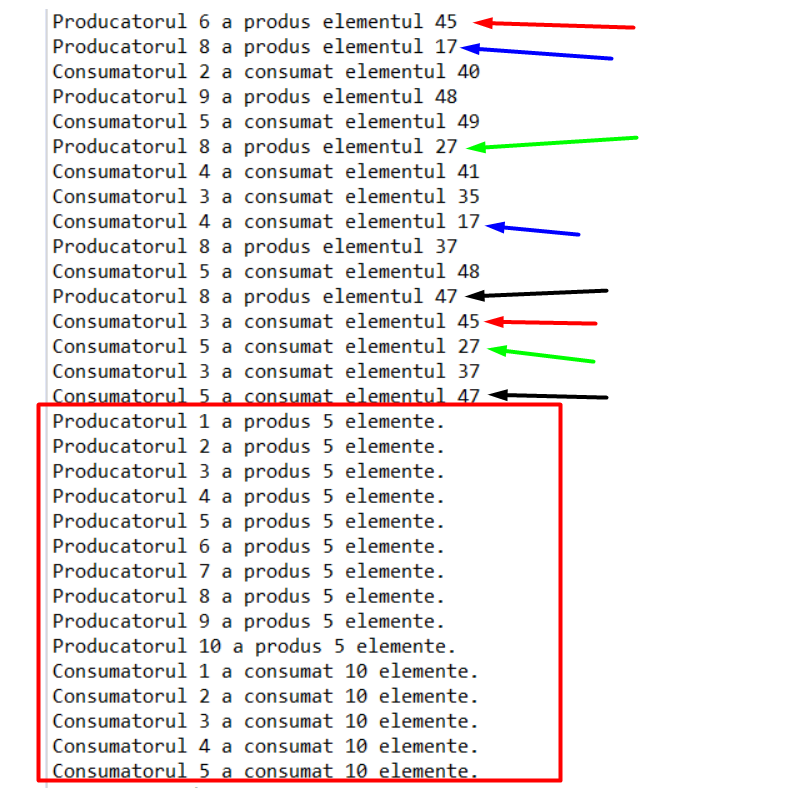
\includegraphics[height=4.3 in, width = 3.5 in]{output_cons.png}
\end{center}

\subsection{\textbf{Concluzii}}

\begin{itemize}
\item Implementand aceasta problema mi-am fixat mai bine cunostintele legate de programarea concurenta, am invatat lucruri noi despre comportamentul firelor de executie cat si despre restrictiile ce ar putea fi aplicate asupra firelor astfel incat rezultatul sa fie cel dorit.

\item Utilizarea mecanismelor de sincronizare este extrem de importanta in programarea concurenta. Studiind aceste mecanisme mi-am imbunatatit abilitatile de programare concurenta.


\item Consider ca aceste tipuri de exercitii au fost foarte bine alese pentru partea aceasta de studiu a mecanismelor de sincronizare ale firelor de executie deoarece implementand solutiile unor  cerinte de acest tip ajungi sa intelegi cu adevarat riscurile executiei unui program pe mai multe fire, stii la ce sa te astepti si cum ai putea rezolva anumite "conflicte" dintre firele de executie.

\end{itemize}

\end{document}
